\chapter{Description générale}
%Décrire les principaux facteurs qui affectent le produit et ses exigences. On n’y énonce pas des exigences spécifiques, mais on y fournit une toile de fond aux exigences qui sont définies en détail à la section 3 afin d’en faciliter la compréhension. Cela comprend les items suivants:

	\section{Perspectives du produit}
%<Describe the context and origin of the product being specified in this SRS. For example, state whether this product is a follow-on member of a product family, a replacement for certain existing systems, or a new, self-contained product. If the SRS defines a component of a larger system, relate the requirements of the larger system to the functionality of this software and identify interfaces between the two. A simple diagram that shows the major components of the overall system, subsystem interconnections, and external interfaces can be helpful.>
L'objectif du produit est de répondre à un besoin d'utiliser une application se conformant à la méthode GTD. De plus, celle ci doit être utilisable en déplacement. Néanmoins il existe déja un certain nombre d'applications GTD de ce type. Cette application est divisée en différents composants. Ce livrable ne concerne cependant que les composants Serveur Web et Client Web (cf. figure \ref{fig:Architecture Generale}), qui nous ont été demandés.


	\section{Fonctions du produit}
%Décrire brièvement les fonctions principales du logiciel. Par exemple : Les fonctions d’un système de gestion peuvent être la maintenance d’un compte client, accéder à l’état de compte du client et produire la facturation.
Le logiciel a pour but de fournir l'ensemble des fonctionnalités décrites dans la méthode GTD. Ces fonctions seront décrites plus précisément dans la suite de ce document.
	
	\section{Caractéristiques et classes d'utilisateurs}
%<Identify the various user classes that you anticipate will use this product. User classes may be differentiated based on frequency of use, subset of product functions used, technical expertise, security or privilege levels, educational level, or experience. Describe the pertinent characteristics of each user class. Certain requirements may pertain only to certain user classes. Distinguish the favored user classes from those who are less important to satisfy.>
Le système sera multi-utilisateur : plusieurs utilisateurs pourront donc se connecter au serveur web. Ces utilisateurs seront à distinguer des administrateurs du serveur GTD disposant de privilèges supérieurs.


	\section{Environnement opérationnel}
%<Describe the environment in which the software will operate, including the hardware platform, operating system and versions, and any other software components or applications with which it must peacefully coexist.>
  \subsection{Matériels}

  Dans un premier temps, l'application serveur sera installée sur une machine d'une puissance minimum, de manière à pouvoir gérer les multiples connexions. Les spécifications de cette machine sont au minimum : \\

  \begin{itemize}
  \item Processeur actuel type Celeron
  \item Mémoire vive de 2go minimum pour gérer les multiples connexions
  \item Disque dur standard
  \end{itemize}

  \medskip

  L'utilisation de notre application sera effectuée à l'aide d'un client web qui par nature sera légé. N'importe quelle configuration permettant l'affichage de pages web sera fonctionnelle :\\

  \begin{itemize}
  \item Processeur actuel type Celeron
  \item Mémoire vive de 1go minimum
  \item Disque dur standard
  \end{itemize}

  \subsection{Système d'exploitation \& client Web}
  En ce qui concerne l'utilisation du service web, elle sera indépendante du système d'exploitation et utilisable avec la pluparts des navigateurs Internet (Firefox, Google Chrome, InternetExplorer ...) 
  
  \medskip
  
  L'application serveur sera quant à elle déployée sur un serveur Linux, et une distribution type Debian ou dérivées.

	\section{Contraintes de conception et d'implémentation}
%<Describe any items or issues that will limit the options available to the developers. These might include: corporate or regulatory policies; hardware limitations (timing requirements, memory requirements); interfaces to other applications; specific technologies, tools, and databases to be used; parallel operations; language requirements; communications protocols; security considerations; design conventions or programming standards (for example, if the customer’s organization will be responsible for maintaining the delivered software).>
Il est impératif de prendre en compte tous les éléments décrits dans la méthode GTD (voir livrable 1). De plus, l'architecture de l'application doit être conforme au schéma suivant : \\

  \begin{figure}[H]
  \begin{center}
  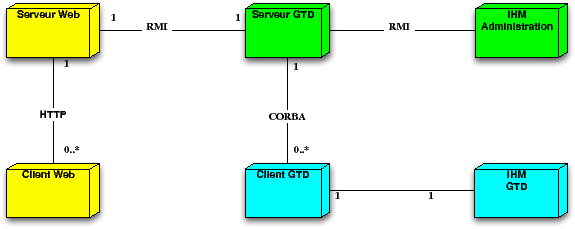
\includegraphics[scale=1]{diagrams/archi.png}
  \caption{Architecture Générale}
  \label{fig:Architecture Generale}
  \end{center}
  \end{figure}



	\section{Documentation utilisateur}
%<List the user documentation components (such as user manuals, on-line help, and tutorials) that will be delivered along with the software. Identify any known user documentation delivery formats or standards.>
Une aide en ligne doit être mise en oeuvre. Une section du site doit être dédiée à celle-ci. Des rollover ou des messages d'aide sur le site guideront l'utilisateur. L'aide en ligne devra  suffir à un utilisateur maitrisant les bases de la navigation Web pour utiliser le logiciel. Aucune aide papier ne sera fournie pour l'application web, de par sa nature distante.


\medskip

Une courte formation sera effectuée lors de la livraison et du déploiement de l'application. Elle sera donnée à l'utilisateur principal du logiciel, lui permettant de la prendre en main rapidement.

	\section{Hypothèses et dépendances}
%Décrire tout élément de faisabilité technique, disponibilité de sous-système ou de composant ou toute autre hypothèse liée au projet de laquelle dépend la viabilité du logiciel.
	
%<List any assumed factors (as opposed to known facts) that could affect the requirements stated in the SRS. These could include third-party or commercial components that you plan to use, issues around the development or operating environment, or constraints. The project could be affected if these assumptions are incorrect, are not shared, or change. Also identify any dependencies the project has on external factors, such as software components that you intend to reuse from another project, unless they are already documented elsewhere (for example, in the vision and scope document or the project plan).>

Comme le montre la figure \ref{fig:Architecture Generale}, l'application est un composite, chaque composant pouvant dépendre d'un autre. Le client Web est ainsi dépendant du serveur Web, qui est lui même dépendant d'un serveur GTD. De même, l'IHM d'administration et le client GTD sont dépendants du Serveur GTD, et l'IHM GTD est dépendante du client GTD.

\medskip

Il sera possible d'utiliser deux serveur GTD. D'une part un server GTD développé par un autre groupe, et d'une autre part un serveur ToodleDo\footnote{www.toodledo.com}.
\section{Exigences reportées}
%Énumérer les exigences qui peuvent être réalisées dans des versions futures du système.
L'internationalisation sera réalisée dans une version future du système. L'application sera fournie en français uniquement dans un premier temps.
